\chapter{Implementatie}

\section{Selectie van de DBMS's}

\subsection{Selectiecriteria voor \glspl{DBMS}}
Bij de selectie van de systemen of een systeem een bepaalde eigenschap al dan niet ondersteunt. In het totaal zijn er 5 verschillende eigenschappen waarop wordt geselecteerd. 

\paragraph{Vrije software} Om testen tussen verschillende \glspl{DBMS} te kunnen vergelijken op een gelijkaardige infrastructuur, is het nodig dat deze software kan geïnstalleerd worden op de eigen infrastructuur. Daarnaast is er in dit onderzoek gekozen voor gratis beschikbare software. 

\paragraph{Persistentie} Voor het testen van de beschikbaarheid van de data, is het een voordeel dat de data op harde schijf aanwezig is: bij herstel dient er minder data over het netwerk gestuurd te worden. Om deze reden hebben deze systemen een voorkeur op systemen die de data enkel in geheugen houden. 

\paragraph{Replicatie} Eén van de testen is de beschikbaarheidstest, indien de data maar op een enkele server opgeslagen is, zal de data op de uitgeschakelde server niet langer beschikbaar zijn. Met replicatie zal de data op verschillende servers opgeslagen worden en zal de data nog steeds beschikbaar zijn in het geval van een enkele uitgeschakelde server. 

\paragraph{Data distributie} Het is de bedoeling om systemen te testen die een grote hoeveelheid data kunnen opslaan. Om aan deze vereiste te voldoen, is het nodig dat elke server niet al de data opslaat bij een voldoende hoog aantal servers (bij weinig servers, is elke server nodig om aan de replicatie vereiste te voldoen)

\paragraph{Ondersteuning voor verschillende query methodes} Bij de testen worden er 5 soorten queries uitgevoerd: invoegen, aanpassen, verwijderen en opvragen van een individueel record en het opvragen van meerdere queries. De \gls{DBMS} moet ondersteuning voor deze queries. De eerste 4 kunnen in al de systemen geïmplementeerd worden met één of meerdere queries. Maar het opvragen van meerdere queries is in bepaalde systemen niet mogelijk en deze worden om deze reden niet behandeld. 

Voor elk van de systemen besproken in sectie \ref{sec:BesprekingDBMS}, is het eerste criterium voldaan voor al deze systemen. De overige 4 criteria zijn samengevat in tabel \ref{table:vergelijkingNosql}. Naast de 4 criteria, is er gekozen om systemen van verschillende klassen te hebben met uitzondering van Key-Value. Samen met mijn collega Arnaud Schoonjans \cite{thesisArnaud}, zijn er in verschillende systemen verder onderzocht. In deze thesis zijn  HBase, MongoDB en Pgpool-II verder onderzocht, in de thesis van mijn collega zijn Cassandra, Apache CouchDB, Riak en MySQL verder onderzocht.  
 
\todo{Update table :-)}
\begin{table}
    \begin{tabular}{lll|l|l|l|l|l|l|l|l|l}
    ~                & ~         & \multicolumn{2}{l}{ \rotatebox[origin=c]{90}{Column database}} & \multicolumn{2}{l}{\rotatebox[origin=c]{90}{Document database}} & \multicolumn{4}{l}{\rotatebox[origin=c]{90}{Key-Value database}} & \multicolumn{2}{l}{\rotatebox[origin=c]{90}{Relationele database}} \\
    ~                & ~         & \rotatebox[origin=c]{90}{Cassandra} & \rotatebox[origin=c]{90}{HBase} & \rotatebox[origin=c]{90}{Apache CouchDB} & \rotatebox[origin=c]{90}{MongoDB} & \rotatebox[origin=c]{90}{Lightcloud (Tokyo)} & \rotatebox[origin=c]{90}{Memcache} & \rotatebox[origin=c]{90}{Riak} & \rotatebox[origin=c]{90}{Voldemort} & \rotatebox[origin=c]{90}{MySQL} & \rotatebox[origin=c]{90}{Pgpool-II (PostgreSQL)} \\
    \multicolumn{2}{l}{Persistentie} & ~               & ~     & ~                 & ~       & ~                  & ~        & ~    & ~         & ~                    & ~                      \\
    \multicolumn{2}{l}{Replicatie} & ~               & ~     & ~                 & ~       & ~                  & ~        & ~    & ~         & ~                    & ~                      \\
    \multicolumn{2}{l}{Data distributie} & ~               & ~     & ~                 & ~       & ~                  & ~        & ~    & ~         & ~                    & ~                      \\
    Query soort      & Aanpassen & ~               & ~     & ~                 & ~       & ~                  & ~        & ~    & ~         & ~                    & ~                      \\
    ~                & Range     & ~               & ~     & ~                 & ~       & ~                  & ~        & ~    & ~         & ~                    & ~                      \\
    \end{tabular}
    \caption{Ondersteuning van de besproken \glspl{DBMS} naar de selectie criteria met de gekozen systemen geaccentueerd.}
    \label{table:vergelijkingNosql}
\end{table}


\section{Gedetailleerde bespreking van de geselecteerde DBMS's}
In dit gedeelte zal elk geselecteerd systemen in meer detail uitgelegd worden, met een focus op de systeem structuur. Een gemeenschappelijk element bij al deze systemen is dat niet alle noden dezelfde functie hebben, in andere \glspl{DBMS} hebben allen dezelfde taak wat de installatie kan vereenvoudigen. 

Voor elk van de geselecteerde systemen zal de aangeboden API besproken worden met een blik op de datastructuur, daarna zal de systeem architectuur besproken worden. 

\subsection{HBase}

\subsubsection{Aangeboden API} \todo{}

\subsubsection{Architectuur}
De gedistribueerde versie van HBase\cite{george2011hbase} is afhankelijk van 2 andere software systemen, namelijk Zookeeper\cite{hunt2010zookeeper} en Hadoop\cite{borthakur2007hadoop}, en volgt hiermee de structuur van Google's BigTable\cite{chang2008bigtable} die op zijn beurt afhankelijk is van Chubby\cite{burrows2006chubby} en Google File System\cite{ghemawat2003google}. Een overzicht van de architectuur bevindt zich in figuur \ref{fig:Hbase-structure}. Deze 3 systemen zullen kort besproken worden, van Hadoop tot Zookeeper en HBase. 

\begin{figure}[h!]
\centering
\includegraphics[width=\linewidth]{img/Hbase-structure.png}
\caption{Volledige systeemarchitectuur van HBase met Hadoop en Zookeeper. Bron \cite{ChinHBaseComprehensive}}
\label{fig:Hbase-structure}
\end{figure}

\paragraph{Hadoop\cite{borthakur2007hadoop}} HBase maakt gebruik van het Hadoop Distributed File System \gls{HDFS}, een gedistribueerd file systeem ontworpen om te werken op commodity hardware met een hoge fout tolerantie. \gls{HDFS} heeft een master/slave architectuur en bestaat uit een enkele \textbf{namenode}, de master server, die de naamruimte en toegangscontrole onderhoudt, en \textbf{datanode}s. De data wordt opgedeeld in blokken die in een verzameling van datanodes wordt opgeslagen, op deze manier is er data distributie en asynchrone replicatie. Deze master/slave configuratie zijn verschillende soorten van services en dient door de gebruiker zelf geconfigureerd te worden. \\
In de configuratie die hier gebruikt wordt, is \gls{HDFS} de methode de data in op te slaan in HBase met automatische replicatie en data distributie. Er is ook nog ondersteuning om dit lokaal op de harde schijf te doen bij een niet distribueerde installatie en om dit weg te schrijven naar S3.\cite{george2011hbase}

\paragraph{Zookeeper\cite{hunt2010zookeeper}} Zookeeper is een service voor het coördineren van gedistribueerde applicatie processen, met deze service biedt primitieven aan om synchronisatie, configuratie onderhoud en groepen en benaming te doen. Zookeeper is op zijn beurt een gedistribueerd master/slave systeem dat ontworpen is om snel te zijn bij dominantie van leesoperaties. De master/slave \\
HBase gebruikt Zookeeper onder andere voor het bijhouden van de status van regio server en hun locatie. \cite{george2011hbase}

\paragraph{HBase\cite{george2011hbase}} HBase is een master/slave systeem welke bestaat uit een HMaster en een HRegionServer. De \textbf{HMaster} is verbonden met Zookeeper en houdt op deze manier de status van de HRegionServers in het oog. Daarnaast is deze ook verantwoordelijk voor het opsplitsen van data (sharding) over verschillende regio's indien een tabel groeit en het toewijzen van een regio aan een HRegionServer.\\
De andere soort, \textbf{HRegionServer}s, is verantwoordelijke voor het dienen en beheren van regio's. Een regio is een deel van een tabel met daarin de feitelijke data die opgeslagen is in verschillende datanodes. Een HRegionServer zal de strikte consistentie afdwingen in HBase, dit kan doordat een enkele server verantwoordelijk is voor het uitvoeren van de data-updates. 

Dit is de globale structuur van het HBase systeem, in het totaal zijn er 5 verschillende soorten systemen, 2 bij Hadoop, 1 bij Zookeeper en 2 bij HBase. Enkele van deze systemen worden best gegroepeerd: de namenode wordt samengesteld met HMaster en een datanode met HRegionServer. Zeker deze laatste heeft een extra performantie invloed: HBase detecteert dat er lokale opslag van de data is en de regio zal steeds deze lokale opslag hebben. Dit gecombineerd met de asynchrone replicatie, zorgt ervoor dat het schrijven van data maar naar een enkele server gestuurd moet worden. 

De configuratie van de verschillende systemen gebeurt door middel van configuratiebestanden voor elke service waarna de volledige configuratie door het systeem zelf wordt gedaan, uitgezonderd het aanmaken van een tabel welke door de API wordt opgezet. 

\subsection{MongoDB}

\subsubsection{Aangeboden API} \todo{}
Bij het schrijven van data, kunnen verschillende eisen gesteld worden voor het voltooien van de actie, startende met de actie is over het netwerk verstuurd, de primary heeft de data geschreven tot een meerderheid van de secundaries heeft de data weg geschreven. \\Bij het lezen kan men kiezen om de data te lezen van de primary, secundary of de dichtstbijzijnde node. Afhankelijk van de gekozen acties, kan er verondersteld worden dat er een verschillende consistentie garantie zal zijn.

\subsubsection{Architectuur}
MongoDB is een \gls{DBMS} dat de vereisten van replicatie en data distributie op een gelaagde manier garandeert. In eerste instantie zal deze de replicatie vereisten invullen, daarna zal hierop horizontale schaalbaarheid ondersteund worden. 

\begin{figure}[h!] 
\centering
	\subfigure[Drie leden van een replica set met een primary en 2 secundaries. ]{\label{fig:mongodb-replicaset} 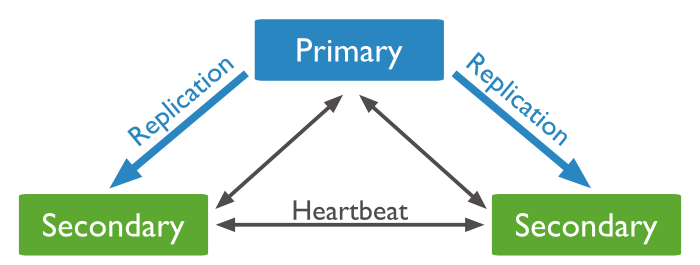
\includegraphics[width=0.40\textwidth]{img/mongodb-replica-set-primary-with-two-secondaries}}
	\hfill
	\subfigure[Een voorbeeld cluster voor productie met 2 mongos, 3 shards en 3 configuratie servers.]{\label{fig:mongodb-sharding} 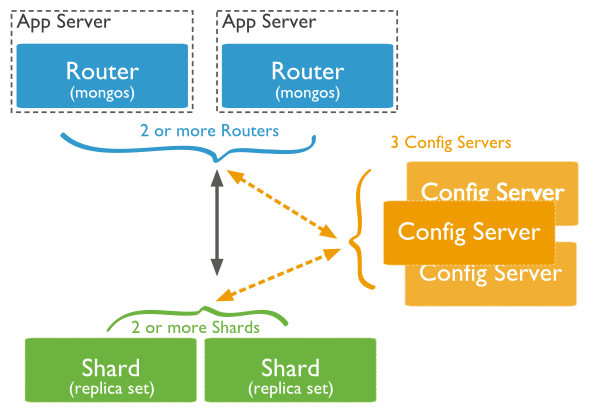
\includegraphics[width=0.50\textwidth]{img/mongo-sharded-cluster-production-architecture}}
	\caption{MongoDB Architectuur voor replicatie en datadistributie. Bron figuur \ref{fig:mongodb-replicaset}: \cite{mongodb-replicaset}, figuur \ref{fig:mongodb-sharding}: \cite{mongodb-shard}}
	\label{fig:mongodb-architectuur}
\end{figure}

\paragraph{Replicatie\cite{mongodb-replicaset}} Replicatie in MongoDB gebeurt door middel van een master/slave configuratie tussen verschillende \textbf{MongoD} instanties, of in hun termen primary/secondundaries. Deze instanties verkiezen zelf hun primary die verantwoordelijk is voor het afhandelen van de schrijfacties, de data zal vervolgens gerepliceerd worden naar de secundaries. Een verzameling van deze MongoD instanties wordt een \textit{replicaset} genoemd. Het is slechts mogelijk om een instantie tot een enkele set toe te voegen. De data is beschikbaar zo lang er meer dan de helft van de servers beschikbaar zijn. 

\paragraph{Data distributie\cite{mongodb-shard}} Horizontale schaalbaarheid wordt in MongoDB aangeboden door verschillende replicaset's of een enkele MongoD instantie te combineren tot een cluster. In het geval van de tweede keuze, zal de data niet gerepliceerd worden en wordt om deze reden niet aangeraden voor productie. 
\subparagraph{Shards} Sharding gebeurt automatisch op een collectie nadat is aangegeven dat men deze wilt verdelen over de gespecificeerde delen. Voor het uitvoeren van deze sharding zijn er nog 2 extra servers types nodig: configuratie servers en toegangsserver. 
\subparagraph{Configuratie servers} De configuratie servers slaan de meta data van de cluster op zoals de verschillende shardings. Deze configuratie set bestaat in productie uit exact 3 servers.
\subparagraph{Toegangsserver} De toegangsserver haalt de configuratie op uit de configuratie servers en biedt toegang voor de gebruiker aan tot de cluster. Er kunnen een onbepaald aantal toegangsservers zijn in cluster. 

De configuratie van de verschillende delen gebeurt op verschillende manieren. Bij replicatie krijgt elke set een naam die in de configuratiebestanden van elke configuratie wordt gezet, nadien wordt via één instantie de verschillende instanties toegevoegd via de API. Bij de cluster worden bij het opstarten van de toegangsservers de set van configuratieservers meegegeven, het opzetten van de verschillende shards gebeurt via een toegangsserver m.b.v. de API. 

\subsection{Pgpool-II (PostgreSQL)}

\subsubsection{Aangeboden API} \todo{}

\subsubsection{Architectuur}

\section{Selectie en uitwerking van de testsoftware}


\section{Installatie van de DBMS's en testsoftware}

%Uitleggen van gebruik van YCSB
\subsection{Automatische installatie met IMP}

\subsubsection{YCSB!}
\subsubsection{HBase}
\subsubsection{MongoDB}
\subsubsection{Pgpool-II (PostgreSQL)}

\section{Uitvoeren van de calibratie en testen}

\section{Verzamelen en analyse van de testresultaten}